\chapter{Framework Architecture}
The repro-tools \todo{name subject to change} is a framework developed for analysing the reproducibility issues occuring in the neuroimages. Though this framework is developed with neuroimaging in focus, it can be used to analyze files belonging to any discipline. In this particular usecase, the HCP data containing the neuroimaging data processed under different conditions is analyzed. The term `condition` here refers to different operating system on which the processing takes place. Under an ideal scenario, different HCP subjects, irrespective of the condition under which the processing takes place, are supposed to have identical checksum. Repro-tool helps in identifying the files having differences by comparing the checksum values. It can also quantify these differences with the help of metrics. Repro-tool can also trace the provenance of these differences with the help of data captured by Reprozip.

\begin{center}
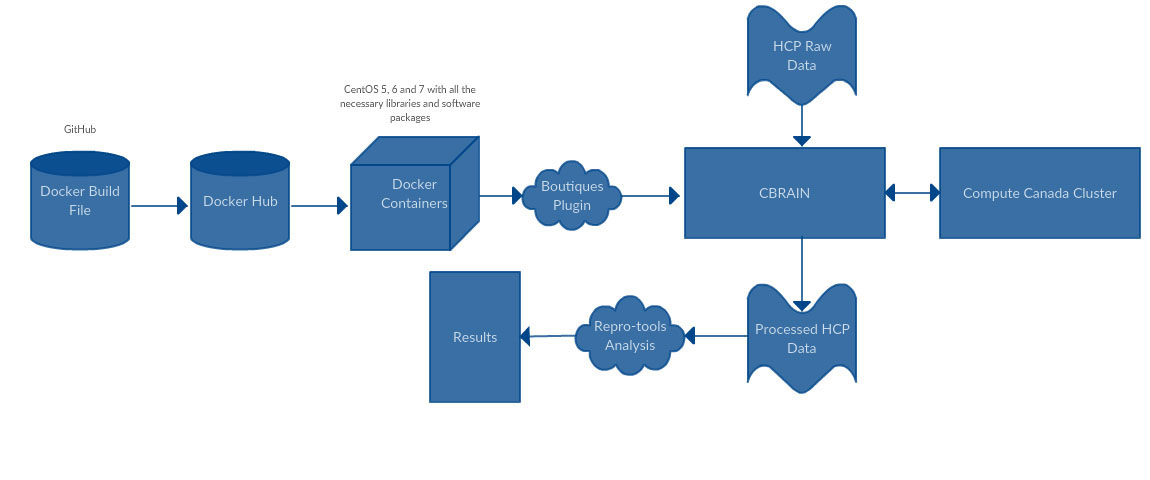
\includegraphics[width=\linewidth]{framework_architecture.jpg}
\captionof{figure}{Framework Architecture}
\label{fig:framework_architecture}
\end{center}

  \begin{itemize}
  \item Collecting data from the Human Connectome Preprocessing Pipelines~\cite{DBHumanConnectome}
  \item Creation of docker images containing the HCP Preprocessing pipelines
  \item Deploying the docker images with the help of Boutiques (A cross-platform application repository for data-analysis platforms) to CBRAIN
  \item Processing of HCP data set using pipelines and measures to check file corruption, recording the software and hardware specifications, provenance capture
  \item Analysis of processed HCP data
  \end{itemize}

\section{Pipeline Containerization}
A container is a self-contained, ready-to-use software component with all the necessary dependencies and softwares~\cite{7158965}. Figure~\ref{fig:container_architecture} illustrates the container image architecture. The architecture is based on LXC which makes use of  cgroups and namespaces. The images are layered on top of each other and the writable container image is kept at the top. The top layer is executable and it can have a state. It can be considered as a directory containing everything needed for exectuion of an application~\cite{7158965}.

\begin{center}
   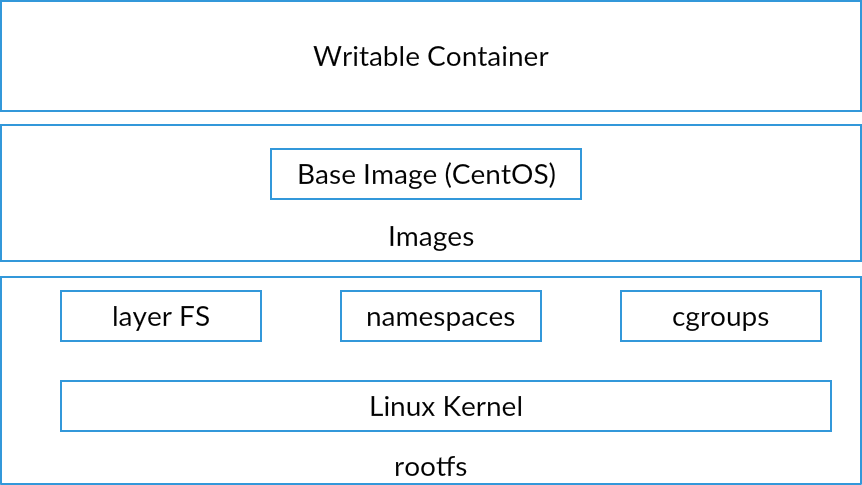
\includegraphics[width=\linewidth]{container_architecture_unedit.png}
   \captionof{figure}{Container Architecture}
   \label{fig:container_architecture}
\end{center}

Namespace isolation prevents processes from seeing resources allocated to each other. Container technologies use seperate namespaces dedicated for each functionality, such as, process isolation, network interfaces, interprocess communication etc. Control groups manage and limit resource access for process groups through limit enforcement, accounting and isolation. Thus namespace and cgroups makes it easier to manage and execute multitenant containers on the host system.

We conducted our study study using Docker containers. A docker image is made up of file systems layered on top of each other using AuFS. The underlying technology is LXC containers. In a traditional Linux boot mechanism, the kernel first mounts the rootfs as read-only, makes the integrity check and changes the rootfs volume permission to read-write mode. Rootfs is, "a simple file system that exports Linux's disk caching mechanisms as a dynamically resizable RAM-based filesystem"~\cite{Rootfs}. But in a Docker container, instead of converting the rootfs to read-write mode, it uses a writable file system as illustrated in~\ref{fig:container_architecture}. 

\subsection{Docker images}
The study of neuroimaging pipelines is conducted on CentOS\footnote{\url{https://en.wikipedia.org/wiki/CentOS}} (Community Enterprise Operating System). According to~\cite{CentOS}, ``CentOS is for people who need an enterprise class operating system stability without the cost of certification and support". CentOS operating system is known for its rock-solid reliability, safety, portability, openness and the long product lifecycle~\cite{5665431}. All these qualities make CentOS a popular choice among the research community and
high performance computing clusters. We conducted our study across the below listed CentOS operating system versions.

\begin{itemize}
  \item Linux CentOS 5.11
  \item Linux CentOS 6.8
  \item Linux CentOS 7.2.1511
\end{itemize}

Docker containers were created out of the base version images listed above. These containers were installed with all the necessary softwares and libraries required to run the HCP pipelines. HCP pipelines prerequisites are listed below,

\begin{itemize}
 \item A 64-bit Linux Operating System
 \item FSL Version - 5.0.6
 \item FreeSurfer Version - 5.3.0-HCP
 \item Connectome Workbench Version - 1.0
 \item HCP version of gradunwarp version 1.0.2 (this is optional and needs to be installed only if gradient nonlinearity corrections needs to be done)
\end{itemize}

We used CentOS 5.11, CentOS 6.8 and Centos7.2.1511 64 bit operating system versions for our study. FSL 5.0.6\footnote{\url{https://fsl.fmrib.ox.ac.uk/fsldownloads/oldversions/}}, FreeSurfer 5.3.0-HCP\footnote{\url{http://ftp.nmr.mgh.harvard.edu/pub/dist/freesurfer/5.3.0-HCP/}} and Connectome Workbench 1.0\footnote{\url{https://www.humanconnectome.org/software/get-connectome-workbench}} were installed in the Docker images.

\subsubsection{HCP Pipelines (v3.19.0)}

\begin{itemize}
  \item FreeSurfer
  \item PreFreesurfer
  \item PostFreeSurfer
  \item fMRIVolume
\end{itemize}

The HCP pipeline is open source, and we used the version 3.19.0 for our study. The details of pipeines are listed below. 
PreFreeSurfer, FreeSurfer and PostFreeSurfer diagrams.

\section{Pipeline Encapsulation}

\begin{itemize}
  \item Describes the command-line interface of the pipeline
  \item Adds checksum to prevent input data corruption
  \item Checks container image identifier
  \item Records all the software (library versions) and hardware specifications
\end{itemize}

\section{Pipeline Deployment}

\begin{itemize}
  \item Single server to ensure no hardware differences
  \item Able to process multiple subjects at once
  \item CBRAIN HCP plugins available here
\end{itemize}

\section{Provenance Capture}

\begin{flushleft}
For every output file, Reprozip captures: 
\end{flushleft}
\begin{itemize}
  \item Process that wrote the file
  \item Command line arguments
  \item Environment variables
  \item Timestamp
  \item Working Directory
\end{itemize}

\section{File comparisions across conditions}

\begin{itemize}
 \item Identify the files that are common to all subjects and all conditions
 \item Check intra-OS variability (e.g., due to pseudo-random processes)
 \item Identifies files with differences (based on md5 checksum)
 \item Associates file types with specific metrics (Normalized RMSE, Text filters, Dice coefficient)
 \item Computes difference matrix for each metric and associates matrix with Reprozip trace
\end{itemize}

\subsection{Metrics}

\begin{itemize}
\item NRMSE
\item Checksum
\item Dice
\item Hardware Differences
\end{itemize}
